\documentclass[ignorenonframetext,]{beamer}
\setbeamertemplate{caption}[numbered]
\setbeamertemplate{caption label separator}{: }
\setbeamercolor{caption name}{fg=normal text.fg}
\beamertemplatenavigationsymbolsempty
\usepackage{lmodern}
\usepackage{amssymb,amsmath}
\usepackage[caption=false]{subfig}
\setbeamertemplate{footline}[frame number]
\usepackage{ifxetex,ifluatex}
\usepackage{fixltx2e} % provides \textsubscript
\ifnum 0\ifxetex 1\fi\ifluatex 1\fi=0 % if pdftex
\usepackage[T1]{fontenc}
\usepackage[utf8]{inputenc}
\else % if luatex or xelatex
\ifxetex
\usepackage{mathspec}
\else
\usepackage{fontspec}
\fi
\defaultfontfeatures{Ligatures=TeX,Scale=MatchLowercase}
\fi
% use upquote if available, for straight quotes in verbatim environments
\IfFileExists{upquote.sty}{\usepackage{upquote}}{}
% use microtype if available
\IfFileExists{microtype.sty}{%
\usepackage{microtype}
\UseMicrotypeSet[protrusion]{basicmath} % disable protrusion for tt fonts
}{}
\newif\ifbibliography

% Prevent slide breaks in the middle of a paragraph:
\widowpenalties 1 10000
\raggedbottom

\AtBeginPart{
\let\insertpartnumber\relax
\let\partname\relax
\frame{\partpage}
}
\AtBeginSection{
\ifbibliography
\else
\let\insertsectionnumber\relax
\let\sectionname\relax
\frame{\sectionpage}
\fi
}
\AtBeginSubsection{
\let\insertsubsectionnumber\relax
\let\subsectionname\relax
\frame{\subsectionpage}
}

\setlength{\parindent}{0pt}
\setlength{\parskip}{6pt plus 2pt minus 1pt}
\setlength{\emergencystretch}{3em}  % prevent overfull lines
\providecommand{\tightlist}{%
\setlength{\itemsep}{0pt}\setlength{\parskip}{0pt}}
\setcounter{secnumdepth}{0}

\title{Opioid Deaths by Race in the United States, 2000--2015}
\subtitle{PAA 2017, Session 133: Trends and Causes of Adult Mortality in the
United States}
\author{Monica Alexander\(^1\) \and Magali Barbieri\(^{1,2}\) \and Mathew Kiang\(^{3}\)}
\institute{\(^1\)University of California, Berkeley \and \(^2\)Institut National d'Etudes Demographiques \and \(^3\)Harvard T.H. Chan School of Public Health}
\date{April 28, 2017}

\begin{document}
\frame{\titlepage}

\begin{frame}{Motivation}

\centering
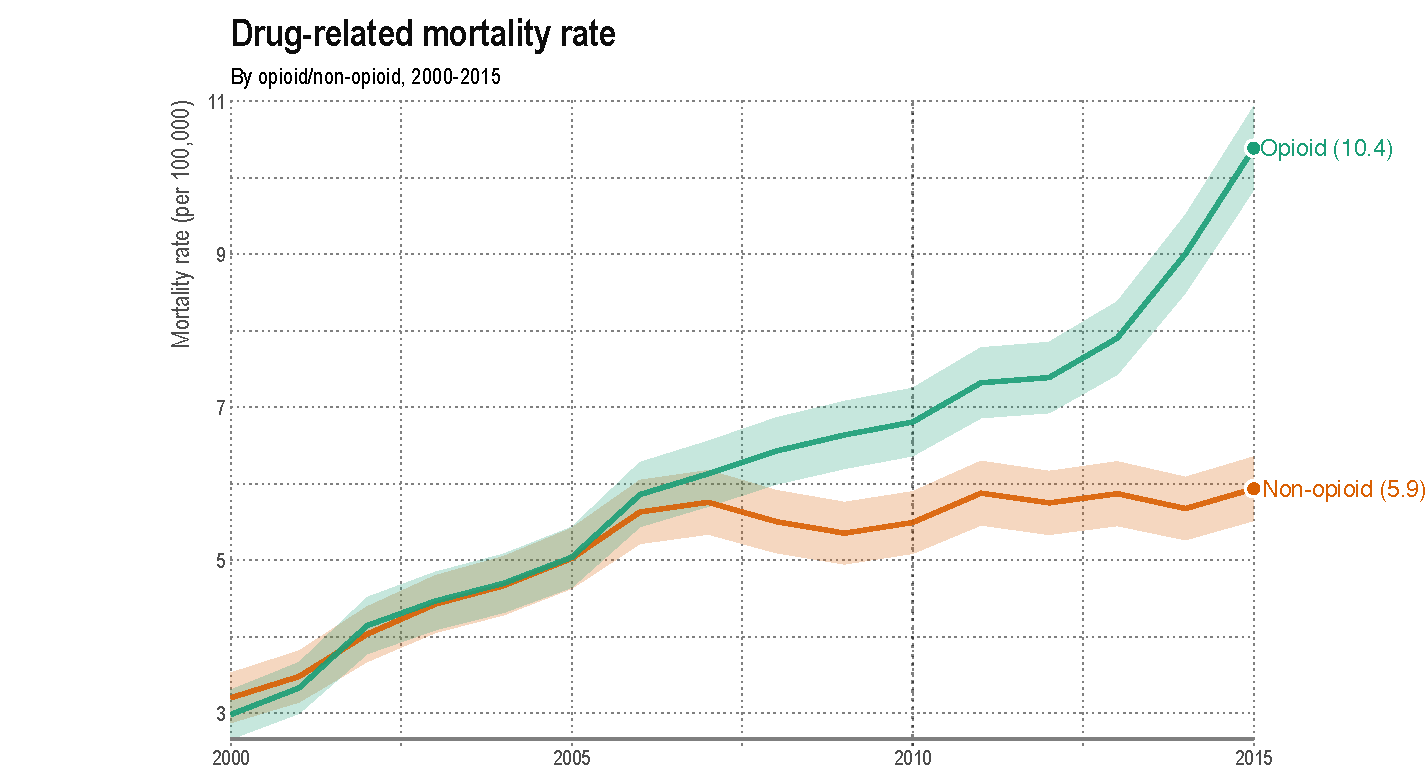
\includegraphics[width=1\textwidth]{./plots/fig1_nood_v_ci.pdf}

\end{frame}

\begin{frame}{Motivation}

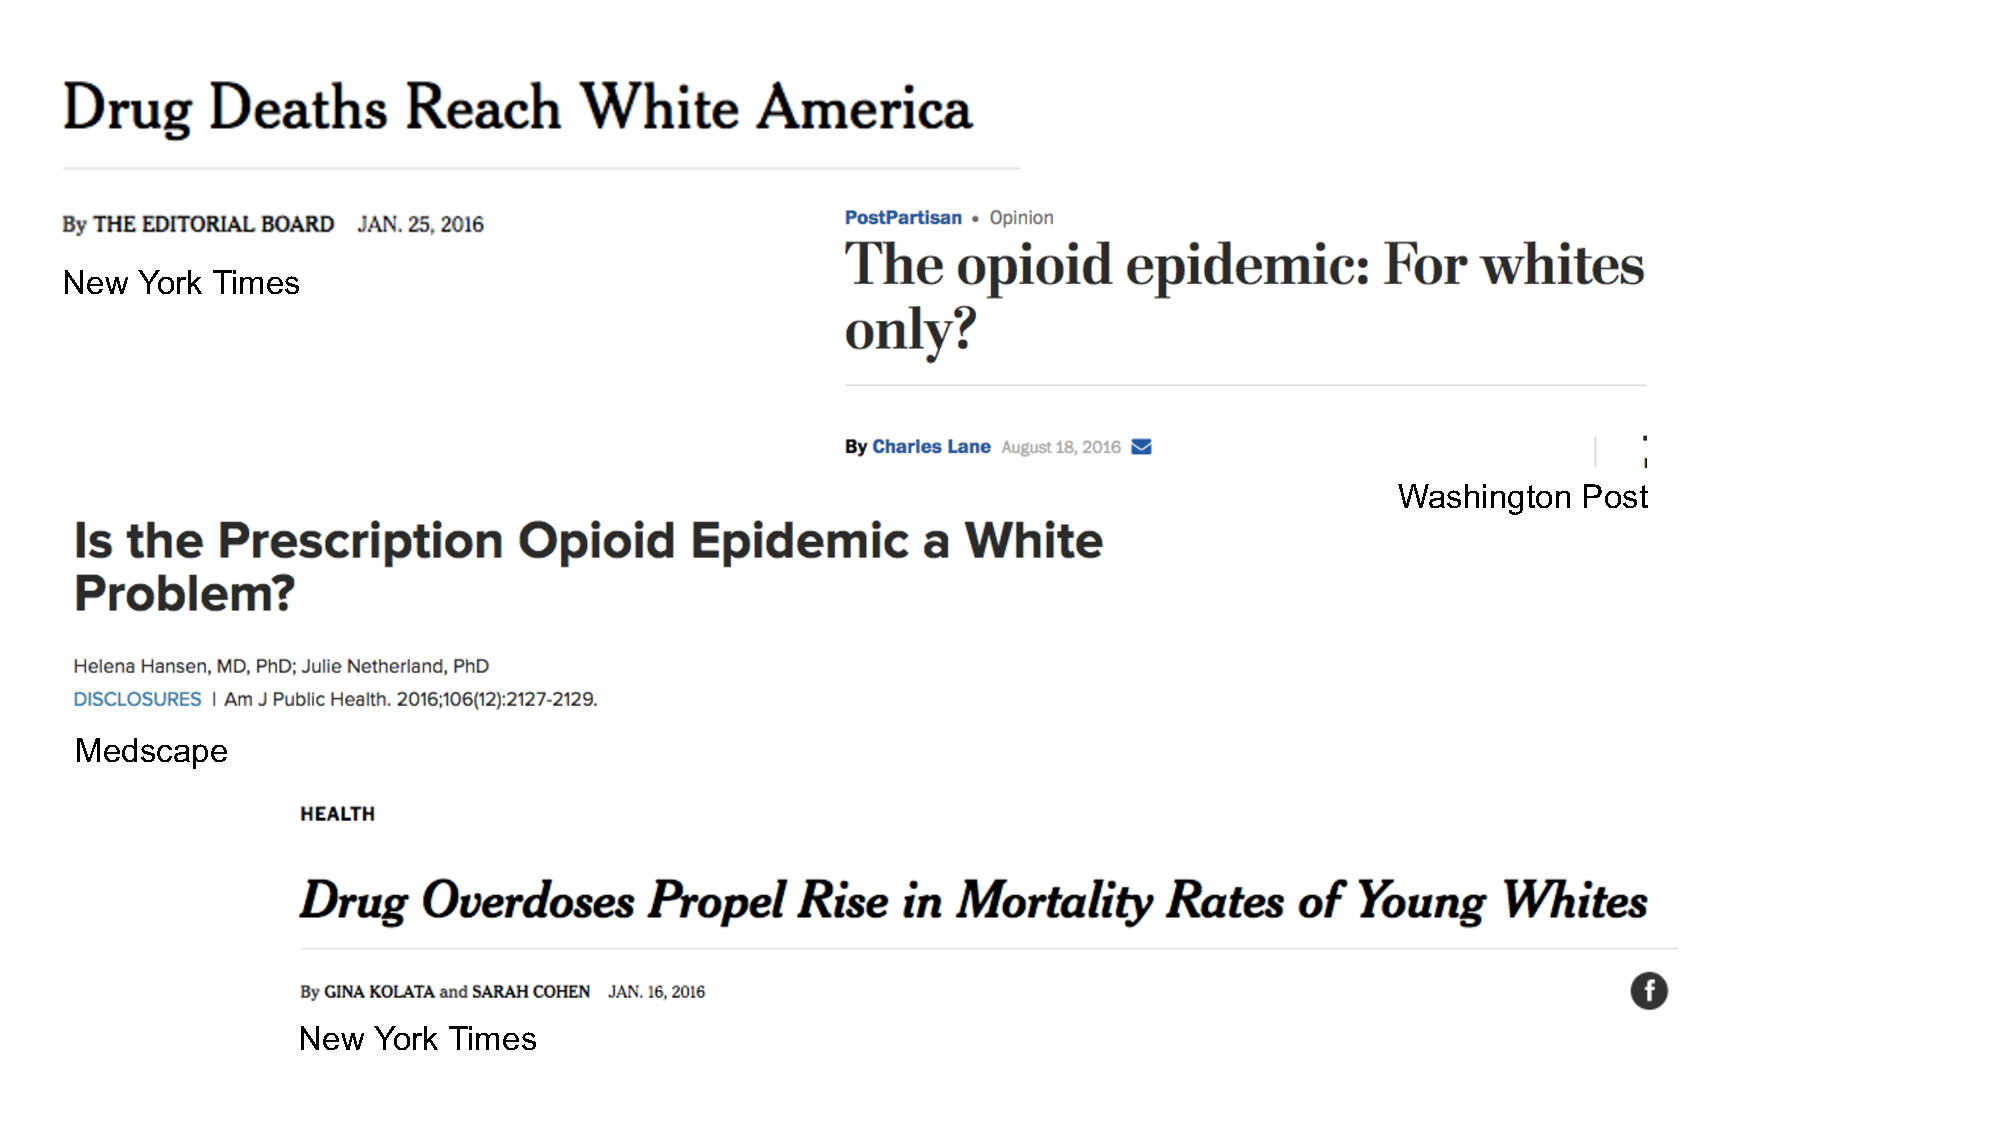
\includegraphics[width=1.25\textwidth]{headline.pdf}

\end{frame}

\begin{frame}{Motivation}


\begin{figure}
\centering
\captionsetup[subfigure]{labelformat=empty}
\subfloat[]{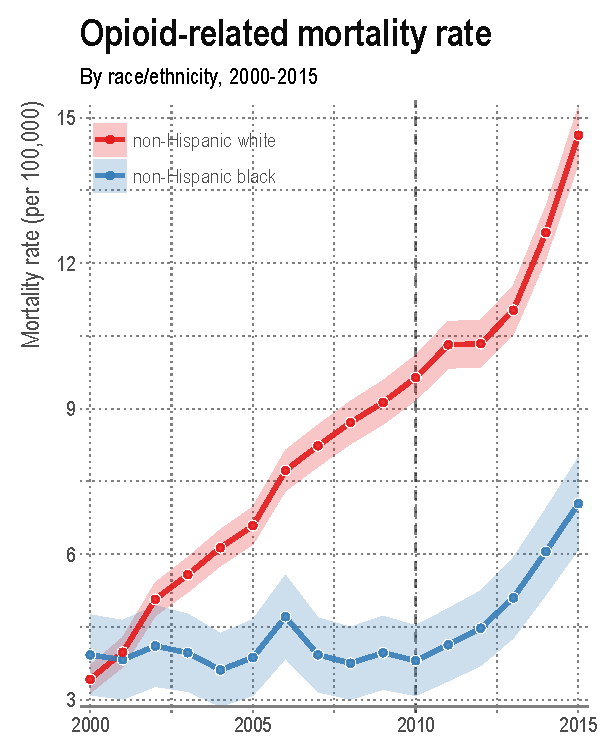
\includegraphics[width=0.47\textwidth]{./plots/fig2_overall_adjusted_ci_v}}
\hfill 
\subfloat[]{\centering 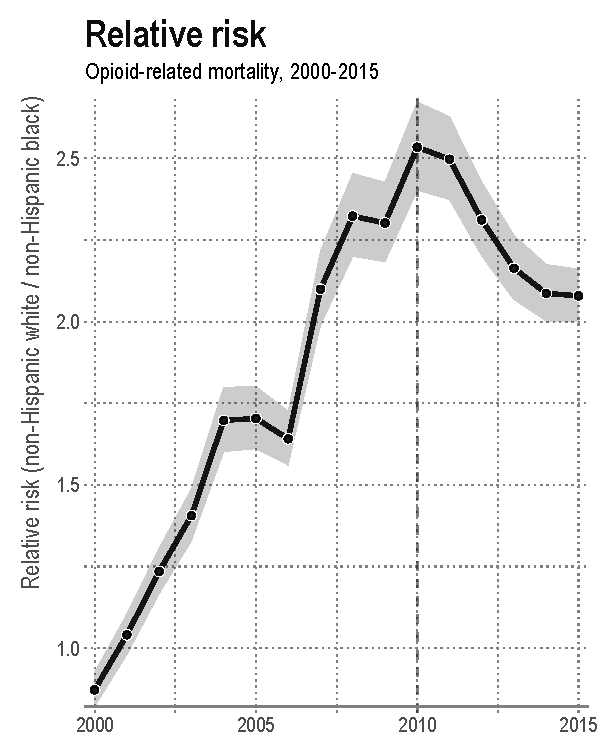
\includegraphics[width=0.47\textwidth]{./plots/fig2_relative_risk_ci_v.pdf}}
\end{figure}
%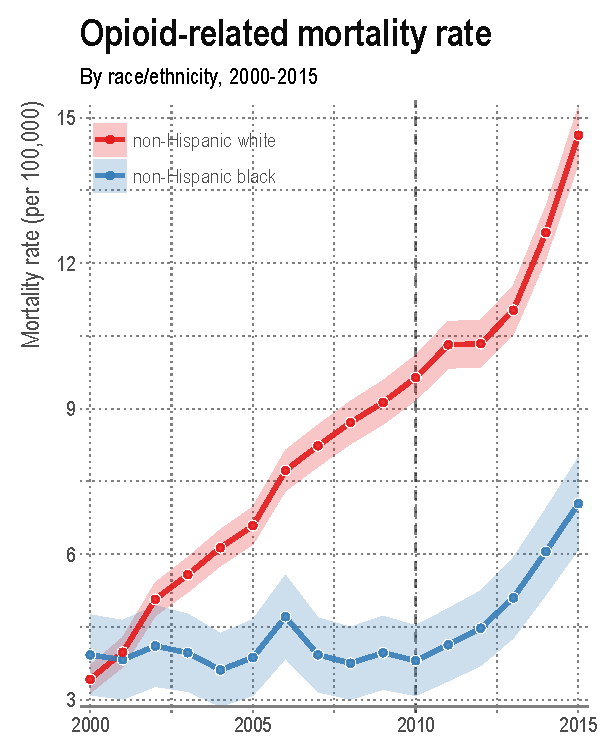
\includegraphics[width=0.5\textwidth]{./plots/fig2_overall_adjusted_ci_v}
%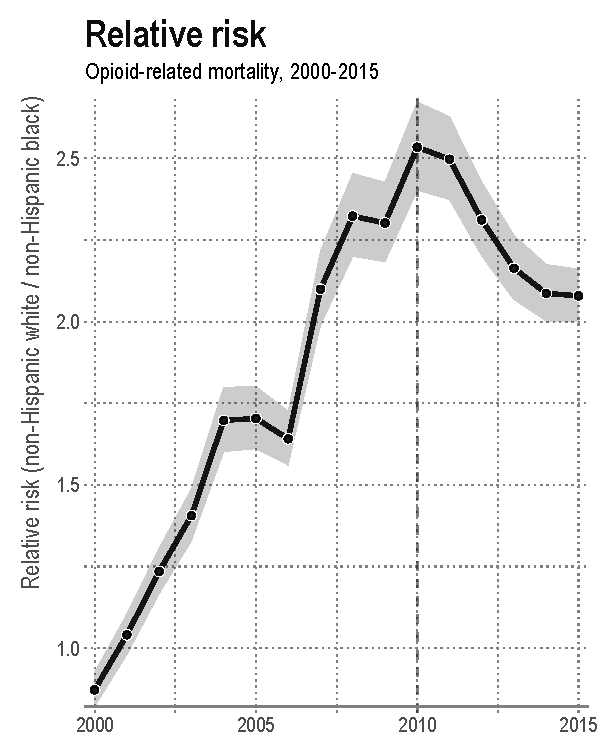
\includegraphics[width=0.5\textwidth]{./plots/fig2_relative_risk_ci_v.pdf}

\end{frame}

\begin{frame}{Aims}

Gain a better understanding how opioid deaths differ \textbf{by race}
and what has contributed to the change in trends over time.

\textbf{Stratify by age} and look at

\begin{itemize}
\tightlist
\item
  Underlying cause of death
\item
  Deaths by opioid type
\item
  Presence of multiple opioids
\end{itemize}

Motivate future research to better target health policy and
rehabilitation programs in different areas and for different
subpopulations.

\end{frame}

\begin{frame}{Data}

\begin{itemize}
\tightlist
\item
  Multiple cause of death microdata, 2000--2015

  \begin{itemize}
  \tightlist
  \item
    Deaths are coded according to ICD-10
  \item
    Underlying cause of death and up to twenty additional contributory
    causes
  \end{itemize}
\item
  Restrict analysis to non-Hispanic white and non-Hispanic black
  populations
\item
  Overall mortality rates are age-standardized using 10-year age groups
  and the 2000 Census population as a standard 
\end{itemize}

\end{frame}

\begin{frame}{Defining opioid-related deaths}

Opioid poisoning T-codes:

\begin{itemize}
\tightlist
\item
  T400: Opium
\item
  T401: Heroin
\item
  T402: Other natural and semi-synthetic opioids
\item
  T403: Methadone
\item
  T404: Other synthetic opioids
\item
  T406: Unspecified
\end{itemize}

\begin{enumerate}
\def\labelenumi{\arabic{enumi}.}
\tightlist
\item
  Drug overdose deaths: combination of T-codes and underlying cause of
  overdose: X40-44, X60-64, Y10-14, X85
\item
  Mental and behavioral complications due to opioid use (F110--F119)
\item
  Other deaths with an opioid T-code as contributory cause
\end{enumerate}

\end{frame}

\begin{frame}{Key findings}

Three key observations came out of analysis:

\begin{enumerate}
\def\labelenumi{\arabic{enumi}.}
\tightlist
\item
  Main type of opioids underlying deaths has shifted
\item
  Age distribution of deaths differs by race
\item
  Presence of multiple opioids has increased
\end{enumerate}

\end{frame}

\begin{frame}{1. Type of opioids underlying deaths has shifted}

\centering
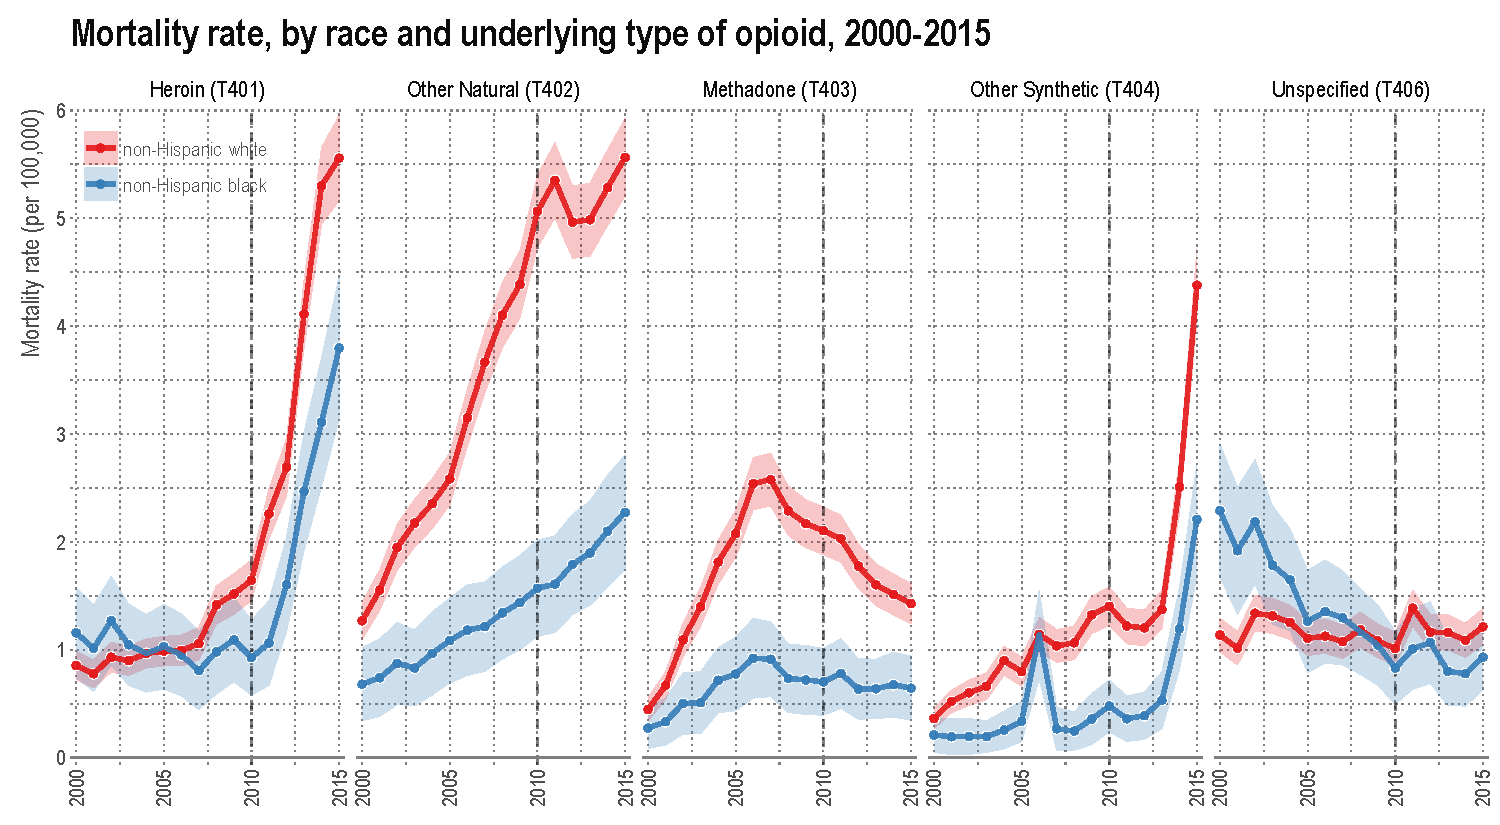
\includegraphics[width=1.0\textwidth]{./plots/fig4_t40_adjusted_race_lines_v_ci.pdf}

\end{frame}

\begin{frame}{2. Age distribution of deaths differs by race}

\centering
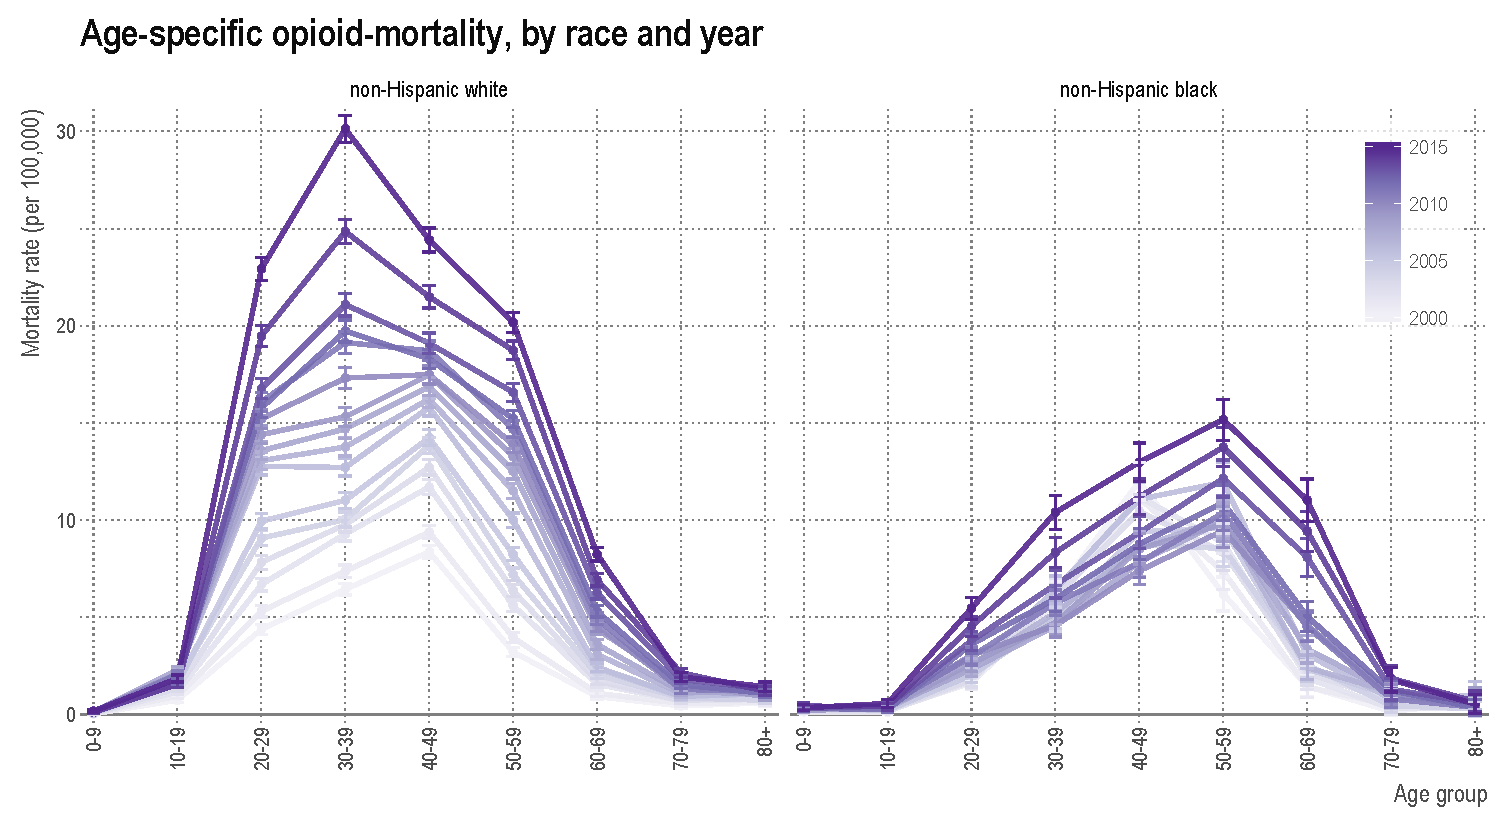
\includegraphics[width=1.0\textwidth]{./plots/fig5_asmr_race_all_errorbars.pdf}

\end{frame}

\begin{frame}{2. Age distribution of deaths differs by race}

\centering
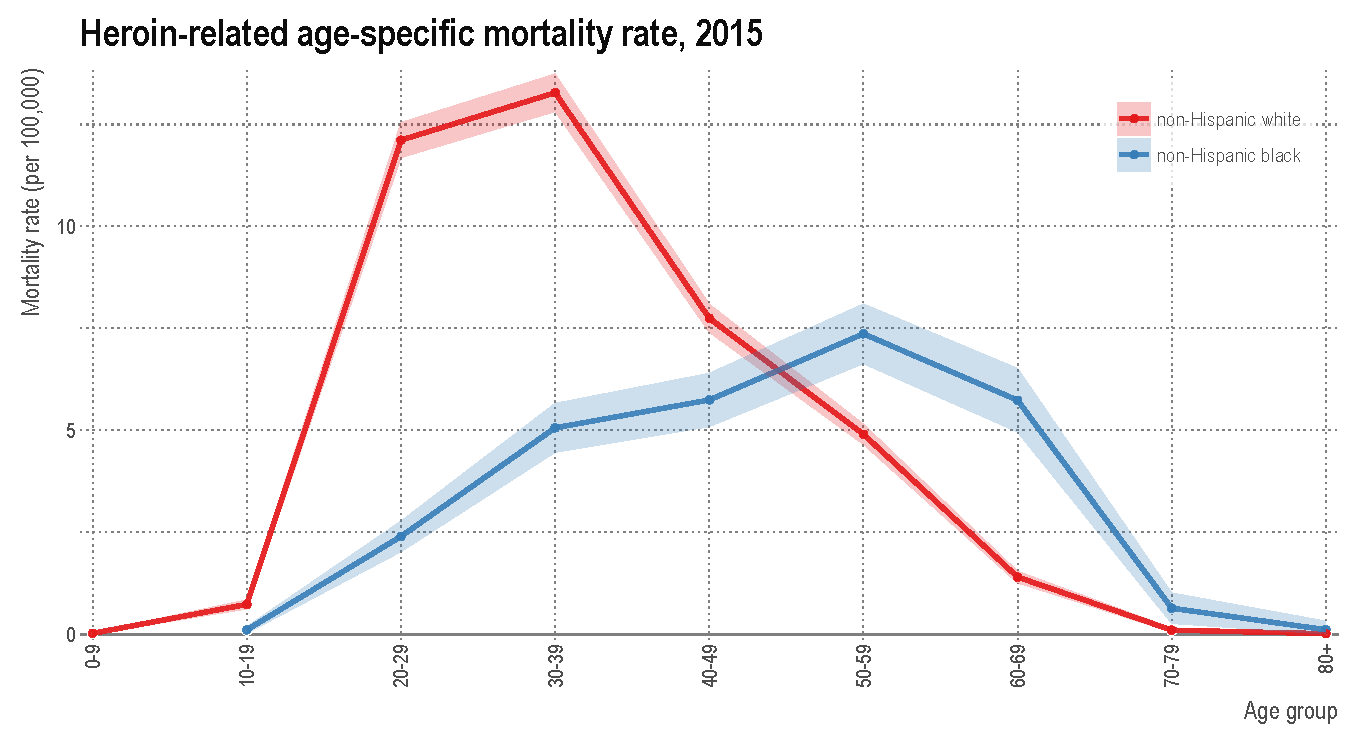
\includegraphics[width=1.0\textwidth]{./plots/fig7_heroin_2015_ci.pdf}

\end{frame}

\begin{frame}{3. Presence of multiple opioids has increased}

\centering
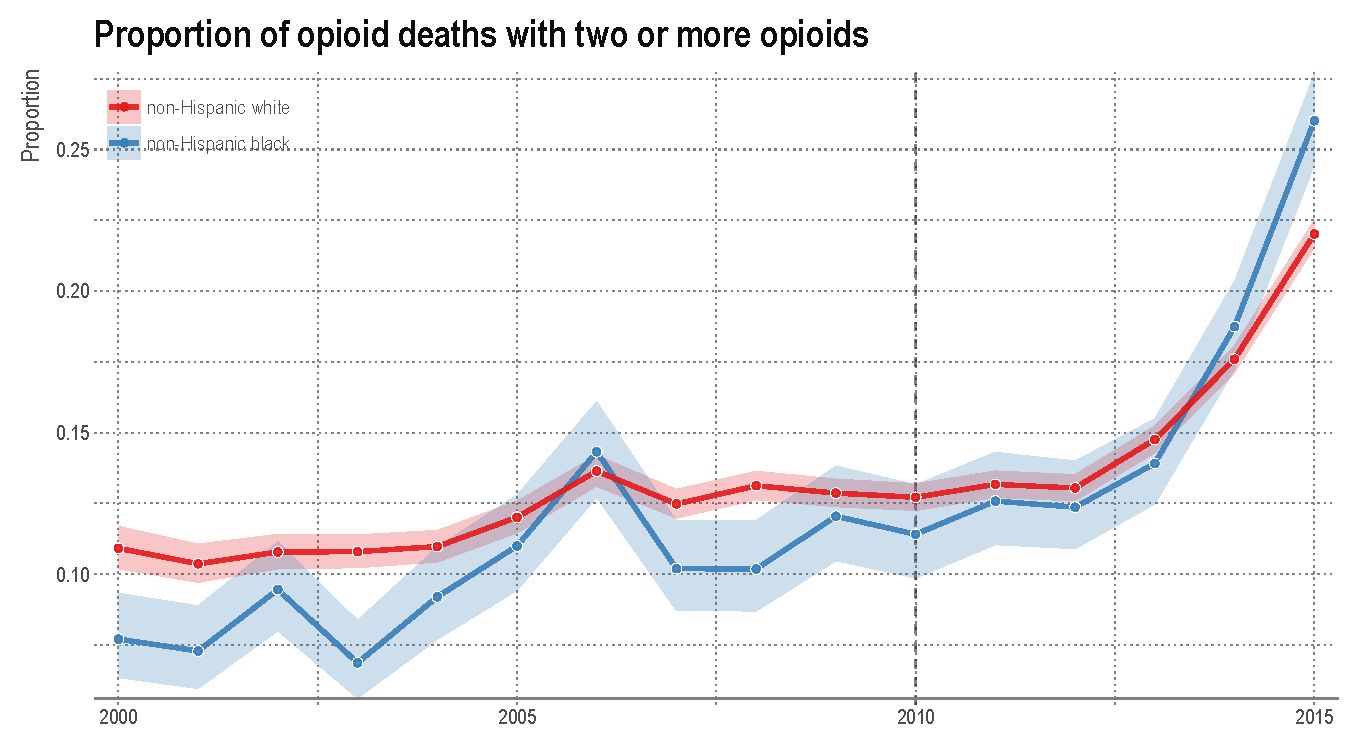
\includegraphics[width=1.0\textwidth]{./plots/fig8_prop_2_more_ci_v.pdf}

\end{frame}

\begin{frame}{3. Presence of multiple opioids has increased}

\centering
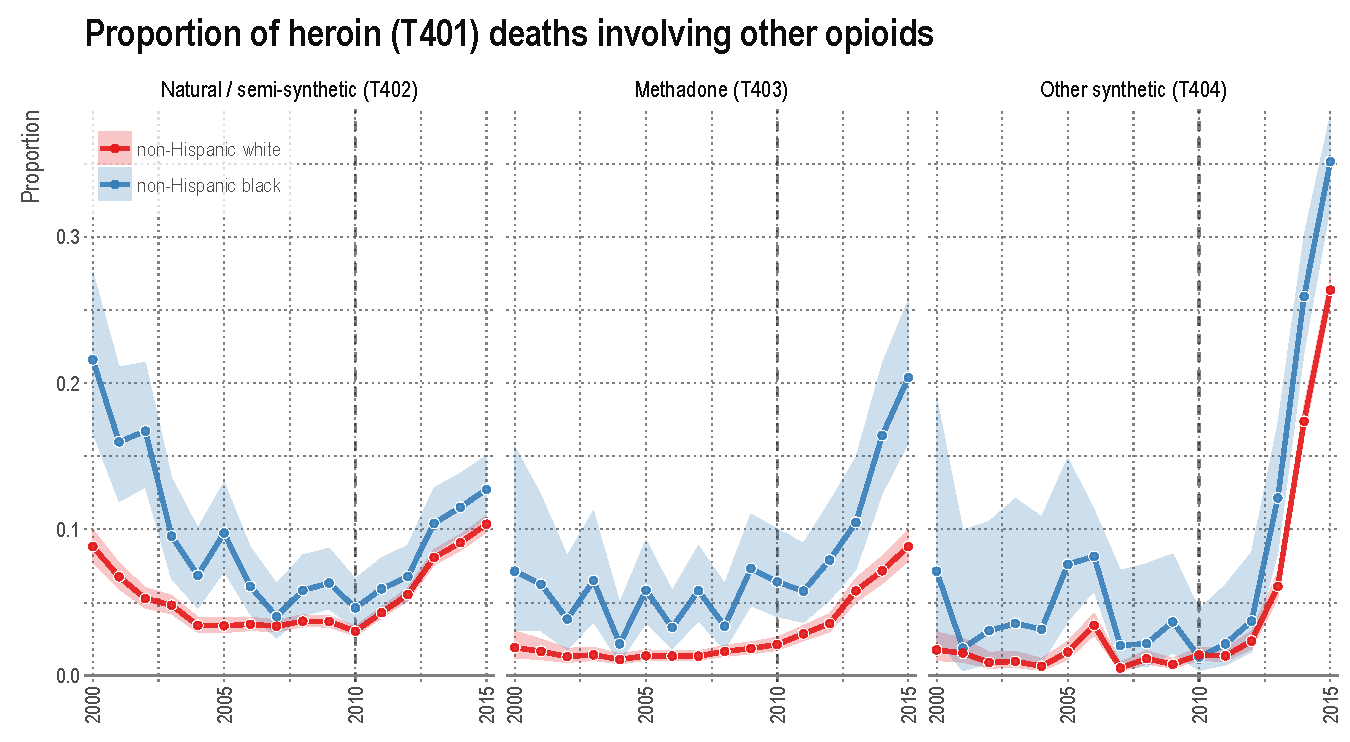
\includegraphics[width=1.0\textwidth]{./plots/fig9_t401_combos_v_ci.pdf}

\end{frame}

\begin{frame}{Summary}

Rising opioid mortality is an issue for both the white and black
populations.

\begin{enumerate}
\def\labelenumi{\arabic{enumi}.}
\tightlist
\item
  The trend in opioid deaths since 2000 has two stages:
\end{enumerate}

\begin{itemize}
\tightlist
\item
  2000--2010: increase for the white population, driven by prescription
  opioids
\item
  2010 onwards: increases for both the white and black populations,
  heroin and fentanyl-related opioids
\end{itemize}

\begin{enumerate}
\def\labelenumi{\arabic{enumi}.}
\setcounter{enumi}{1}
\tightlist
\item
  Much of the increase in deaths due to heroin and fentanyl has occurred
  from a mixture of both drugs.
\item
  White population exhibits a comparatively younger age profile.
\end{enumerate}

\end{frame}

\begin{frame}{Questions / future work}

\begin{enumerate}
\def\labelenumi{\arabic{enumi}.}
\tightlist
\item
  How much of increase in heroin mortality is due to increased use
  versus increased potency?
\item
  What is driving the differences in age by race?
\end{enumerate}

Drawing on:

\begin{itemize}
\tightlist
\item
  More detailed multiple cause of death data with residence information
\item
  Data on prescriptions dispensed and drug use (e.g.~National Survey of
  Drug Use and Health)
\end{itemize}

\end{frame}

\begin{frame}{Thanks!}

Code to reproduce graphs can be found here:
\url{https://github.com/MJAlexander/opioid-mcd}

\begin{figure}
\captionsetup[subfigure]{labelformat=empty}
\subfloat[]{
\includegraphics[width=0.25\textwidth]{demogseal2.png}}
\par\vfill \vspace{-0.5cm}
\subfloat[]{\centering 
\includegraphics[width=0.7\textwidth]{HarvardChan_logo_hrz_RGB.pdf}}
\end{figure}

%
\includegraphics[width=0.2\textwidth]{demogseal2.png}
%
\includegraphics[width=0.7\textwidth]{HarvardChan_logo_hrz_RGB.pdf}

\end{frame}

\end{document}
